\documentclass{article}
\usepackage[utf8]{inputenc}
\usepackage{graphicx}
\usepackage{listings}
\usepackage{color}
\usepackage{geometry}
\geometry{a4paper, margin=1in}

\definecolor{codegreen}{rgb}{0,0.6,0}
\definecolor{codegray}{rgb}{0.5,0.5,0.5}
\definecolor{codepurple}{rgb}{0.58,0,0.82}
\definecolor{backcolour}{rgb}{0.95,0.95,0.92}

\lstdefinestyle{mystyle}{
    backgroundcolor=\color{backcolour},   
    commentstyle=\color{codegreen},
    keywordstyle=\color{magenta},
    numberstyle=\tiny\color{codegray},
    stringstyle=\color{codepurple},
    basicstyle=\ttfamily\footnotesize,
    breakatwhitespace=false,         
    breaklines=true,                 
    captionpos=b,                    
    keepspaces=true,                 
    numbers=left,                    
    numbersep=5pt,                  
    showspaces=false,                
    showstringspaces=false,
    showtabs=false,                  
    tabsize=2
}

\lstset{style=mystyle}

\title{HW7 Report}
\author{Yu Xiang Luo, B10902037}
\date{\today}

\begin{document}

\maketitle

\section{Introduction}
This report describes a Python script developed to perform image thinning using the morphological thinning algorithm. The script applies iterative conditional marking to reduce the thickness of the shapes in a binary image to a single pixel width.

\section{Algorithm Description}
The script executes an image thinning algorithm, which is a morphological operation that is used to remove selected foreground pixels from binary images. It iteratively erodes away the boundaries of regions of foreground pixels (usually white on a black background) until only minimal pixel width lines remain.

\section{Code Implementation}
The code is written in Python, using the Pillow library for image manipulation. The algorithm consists of several functions:

\begin{itemize}
    \item \texttt{ds(image, sfac)}: Downsamples the image by a scaling factor.
    \item \texttt{get\_np(image, position)}: Retrieves a 3x3 neighborhood of pixels around a specified position.
    \item \texttt{hf(b, c, d, e)}: Applies a condition function based on pixel values.
    \item \texttt{ff(a1, a2, a3, a4)}: Determines the action based on conditions returned by \texttt{hf}.
    \item \texttt{get\_yn(image)}: Generates a matrix based on conditions applied to each pixel.
    \item \texttt{get\_im(yn)}: Creates an image from the condition matrix.
    \item \texttt{dilation(image)}: Performs the dilation operation on the image.
    \item \texttt{get\_tm(image, yn, dm)}: Applies thinning to the image.
\end{itemize}

\subsection{Code Snippet}
Below is a snippet from the script showing the main loop of the thinning process:

\begin{lstlisting}[language=Python]
# Main loop of the thinning process
while True:
    yn = get_yn(tm)
    im = get_im(yn)
    dm = dilation(im)
    tmp = get_tm(tm, yn, dm)
    if ImageChops.difference(tmp, tm).getbbox() is None:
        break
    tm = tmp
    Iter += 1
    print(f'Iteration: {Iter}')
tm.save(f'./img/thinning{Iter}.bmp')
\end{lstlisting}

\section{Results}
The algorithm was applied to a binary image, and the process was iterated until no further changes were observed. The final result is a thinned version of the original image, with all objects reduced to single-pixel width.

\subsection{Thinning Process Image}
Below is the thinned image after the final iteration of the algorithm:

\begin{figure}[h]
    \centering
    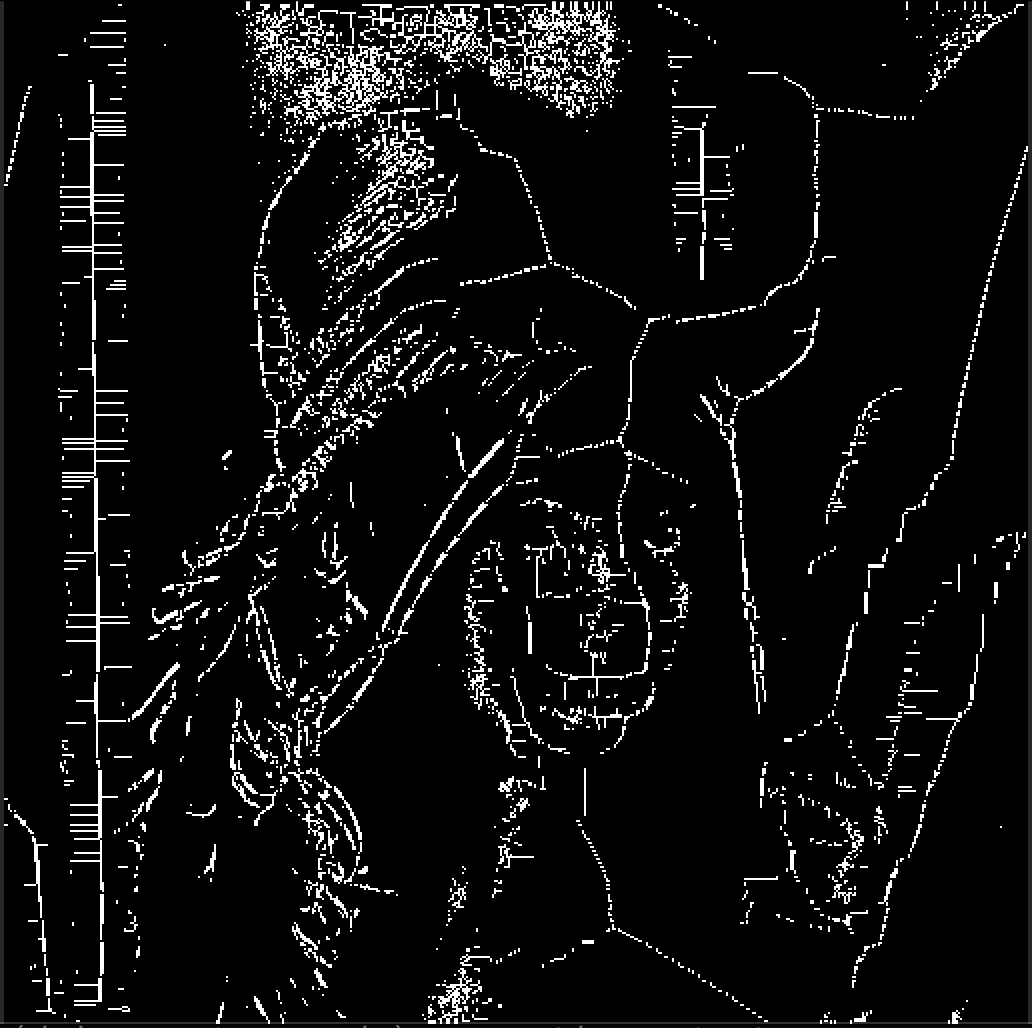
\includegraphics[width=0.5\textwidth]{./img/thinningIter.png}
    \caption{The binary image after the thinning process.}
    \label{fig:thinningIter}
\end{figure}

\section{Conclusion}
The implemented thinning algorithm successfully reduces the objects in a binary image to single pixel width lines. This can be particularly useful for applications in pattern recognition, image processing, and computer vision where the structure of objects is to be analyzed without the influence of varying object thickness.

\end{document}

